% Please use LuaLaTeX or XeLaTeX for compilation
\documentclass[11pt,aspectratio=169]{beamer}

% Theme and Colors
\usetheme{eth}
\colorlet{titlefgcolor}{ETHGray}
\colorlet{accentcolor}{ETHRed}
\colorlet{titlebgcolor}{ETHRed} % Title slide background

% Standard Packages
\usepackage{amsmath, amssymb} % Math symbols
\usepackage{bm} % Bold math symbols
\usepackage{graphicx} % Include graphics (if needed)
\usepackage{booktabs} % Nicer tables (if needed)
\usepackage{microtype} % Better typography
\usepackage{physics} % Physics notation

% Ben packages
\usepackage{soul}

% Citation Management (using biblatex)
\usepackage[style=numeric, backend=biber]{biblatex}
\addbibresource{references.bib} % You need a references.bib file

% Footnotes (optional, if needed)
\usepackage[multiple]{footmisc}
\usepackage{footnoterange}
\usepackage{fnpct}
\AdaptNote\footcite{oo+m}[footnote]{%
\setfnpct{dont-mess-around}%
\IfNoValueTF{#1}
{#NOTE{#3}}
{\IfNoValueTF{#2}{#NOTE[#1]{#3}}{#NOTE[#1][#2]{#3}}}%
}

% Algorithms (optional, if needed)
\usepackage{algorithm}
\usepackage[noend]{algpseudocode} % Use noend option as in template

% Tikz/PGFPlots (optional, if needed for diagrams)
\usepackage{tikz}
\usetikzlibrary{shapes, arrows, positioning, calc}
\usepackage{pgfplots}
\pgfplotsset{compat=1.17} % Use a recent compatibility level

% Custom command for highlighting math
\newcommand\mathalert[1]{{\color{accentcolor}#1}}

% --- Presentation Metadata ---
\title{The Berezinskii-Kosterlitz-Thouless Transition in the 2D XY Model}
\subtitle{Monte Carlo Simulation and Analysis}
\author{Lara Turgut \and Francesco Conoscenti \and Ben Bullinger}
\institute{ETH Zürich\\ Department of Physics}
\date{Computational Statistical Physics (402-0812-00L), Spring 2025}

\begin{document}

% --- Title Slide ---
\def\titlefigure{} % No figure on title slide unless specified
\setlength{\titleboxwidth}{0.85\textwidth} % Adjust box width if needed
\titleframe % Creates the title slide using the theme's definition

% --- Table of Contents ---
\tocframe % Creates the table of contents slide

% --- Section 1: Introduction ---
\section{Introduction}

\begin{frame}{The 2D XY Model}
    \begin{itemize}
        \item XY model: classical spins on a 2D lattice, constrained to a plane with $O(2)$ symmetry.
        \begin{equation*}
            H = -J \sum_{\langle i,j \rangle} \mathbf{S}_i \cdot \mathbf{S}_j = -J \sum_{\langle i,j \rangle} \cos(\theta_i - \theta_j)
        \end{equation*}
        \item Each spin is a unit vector $\mathbf{S}_i = (\cos\theta_i, \sin\theta_i)$. $J>0$ favors alignment.
        \item Control parameter: Temperature $T$. We study behavior as $T$ varies.
        \pause
        \item Unlike conventional phase transitions with symmetry breaking:
            \begin{itemize}
                \item \textbf{Mermin-Wagner theorem:} No spontaneous breaking of continuous symmetries (hence no true long-range order) at $T > 0$ in $d \leq 2$.
                \item Yet, the 2D XY model \textit{does} exhibit a phase transition!
            \end{itemize}
        \pause
        \item The Berezinskii-Kosterlitz-Thouless (BKT) transition:
            \begin{itemize}
                \item Topological phase transition with no conventional order parameter.
                \item Transition from quasi-long-range order (QLRO) to exponential disorder.
                \item Driven by the unbinding of vortex-antivortex pairs.
            \end{itemize}
    \end{itemize}
\end{frame}

\begin{frame}{Physical Significance}
    \begin{itemize}
        \item The BKT transition represents a unique phase transition mechanism
        \begin{itemize}
            \item \textbf{Infinite-order transition:} All derivatives of free energy are continuous
            \item \textbf{Topological in nature:} Driven by topological defects (vortices)
        \end{itemize}
        \pause
        \item Found in diverse physical systems:
        \begin{itemize}
            \item Thin films of superfluid helium-4
            \item 2D superconductors
            \item 2D melting (KTHNY theory)
            \item Josephson junction arrays
            \item Cold atom systems
            \item Quantum spin systems
        \end{itemize}
        \pause
        \item Universal mechanism: A beautiful example of universality in critical phenomena
    \end{itemize}
\end{frame}

% --- Section 2: Theoretical Background ---
\section{Theoretical Background}

\begin{frame}{Algebraic Order in the 2D XY Model}
    \begin{itemize}
        \item Spin-wave approximation (valid at low temperature):
        \begin{equation*}
            H \approx E_0 + \frac{J}{2} \int d^2r (\nabla \theta(\mathbf{r}))^2
        \end{equation*}
        \pause
        \item Correlation function analysis within this approximation yields:
        \begin{equation*}
            g(r) = \langle e^{i(\theta(\mathbf{r}) - \theta(0))} \rangle \approx \left( \frac{r}{a} \right)^{-\eta(T)} \quad \text{with} \quad \eta(T) = \frac{k_B T}{2\pi J}
        \end{equation*}
        \item Key property: \mathalert{Algebraic decay} of correlations at low temperature.
        \begin{itemize}
            \item \textbf{Low-T phase (QLRO):} $g(r) \sim r^{-\eta(T)}$ with temperature-dependent exponent.
            \item \textbf{High-T phase (Disordered):} $g(r) \sim e^{-r/\xi(T)}$ (exponential decay).
        \end{itemize}
        \pause
        \item This algebraic decay = \textbf{Quasi-Long-Range Order (QLRO)}.
        \begin{itemize}
            \item Infinite correlation length $\xi = \infty$ in the low-T phase.
            \item System is critical at all temperatures below $T_{KT}$.
        \end{itemize}
    \end{itemize}
\end{frame}

\begin{frame}{The Role of Vortices}
    \begin{itemize}
        \item Vortices: topological defects with winding of $2\pi n$ in phase field
        \begin{equation*}
            \oint \nabla \theta \cdot d\mathbf{l} = 2\pi n
        \end{equation*}
        \item Energy of a single vortex (with $n=1$):
        \begin{equation*}
            \Delta E = \pi J \ln \frac{L}{a}
        \end{equation*}
        where $L$ is system size and $a$ is lattice spacing
        \pause
        \item Entropy of a single vortex:
        \begin{equation*}
            \Delta S = k_B \ln \frac{L^2}{a^2} = 2k_B \ln \frac{L}{a}
        \end{equation*}
        \pause
        \item Free energy:
        \begin{equation*}
            \Delta F = \Delta E - T\Delta S = (\pi J - 2k_B T)\ln \frac{L}{a}
        \end{equation*}
        \pause
        \item \mathalert{Crucial insight}: Vortices are bound in pairs below critical temperature, and unbound above it
        \begin{itemize}
            \item For $T < \frac{\pi J}{2k_B}$: $\Delta F > 0$ (bound vortex pairs)
            \item For $T > \frac{\pi J}{2k_B}$: $\Delta F < 0$ (free vortices proliferate)
        \end{itemize}
    \end{itemize}
\end{frame}

% --- NEW FRAME FOR VISUALIZATION ---
\begin{frame}{Visualizing Spin Configurations and Vortices}
    \begin{columns}[T] % Use columns to place images side-by-side
        \begin{column}{0.33\textwidth}
            \centering
            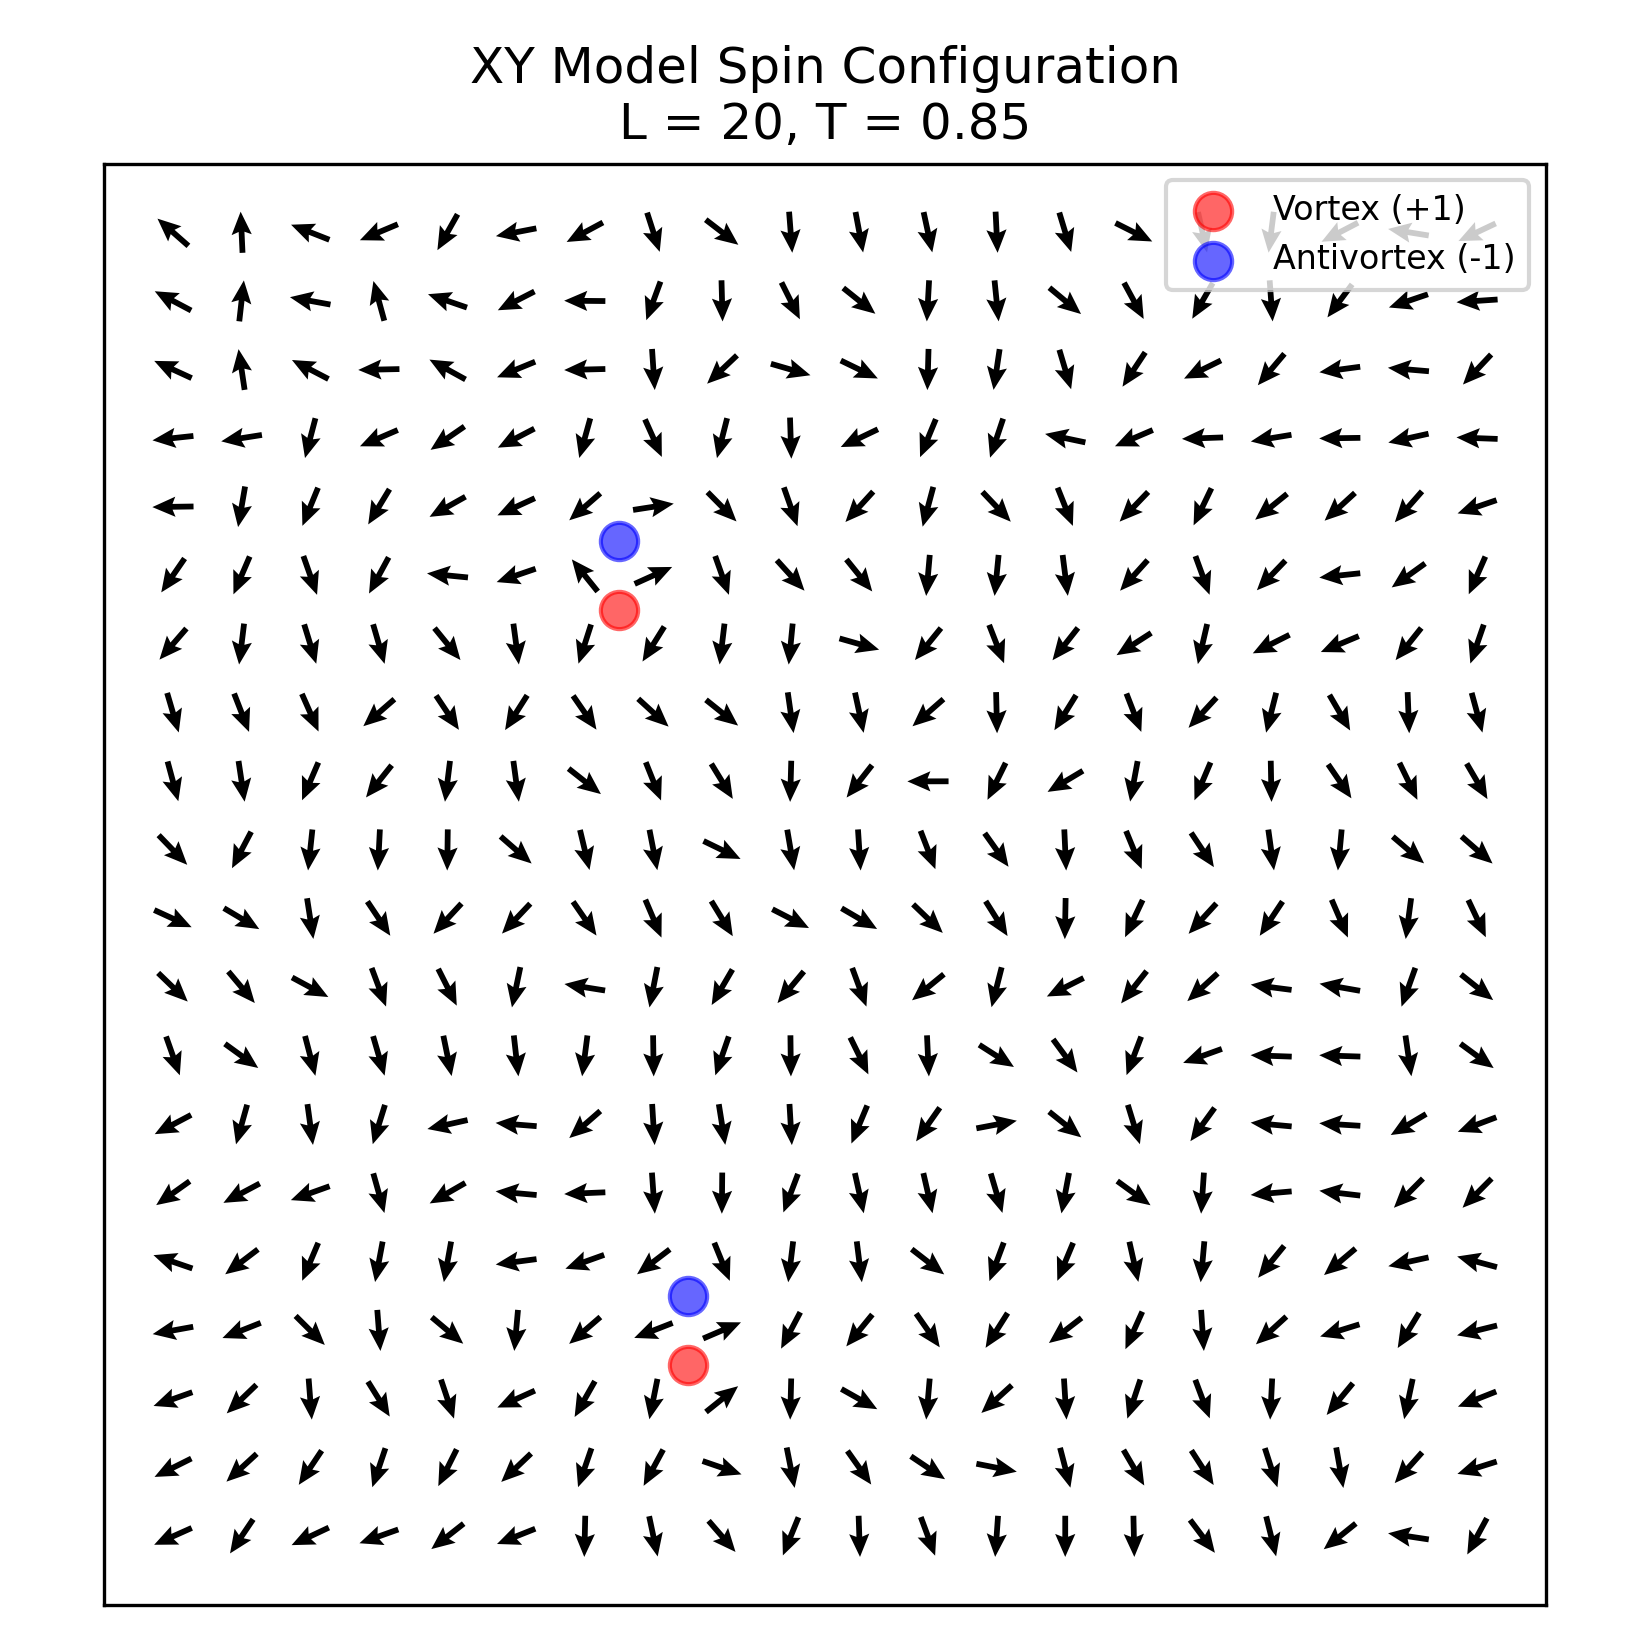
\includegraphics[width=\linewidth]{images/visualization/xy_model_L20_T0.85_vis.png}
            \tiny $T = 0.85 \lesssim T_{KT}$\\(QLRO, Approaching Transition)
        \end{column}
        \begin{column}{0.33\textwidth}
            \centering
            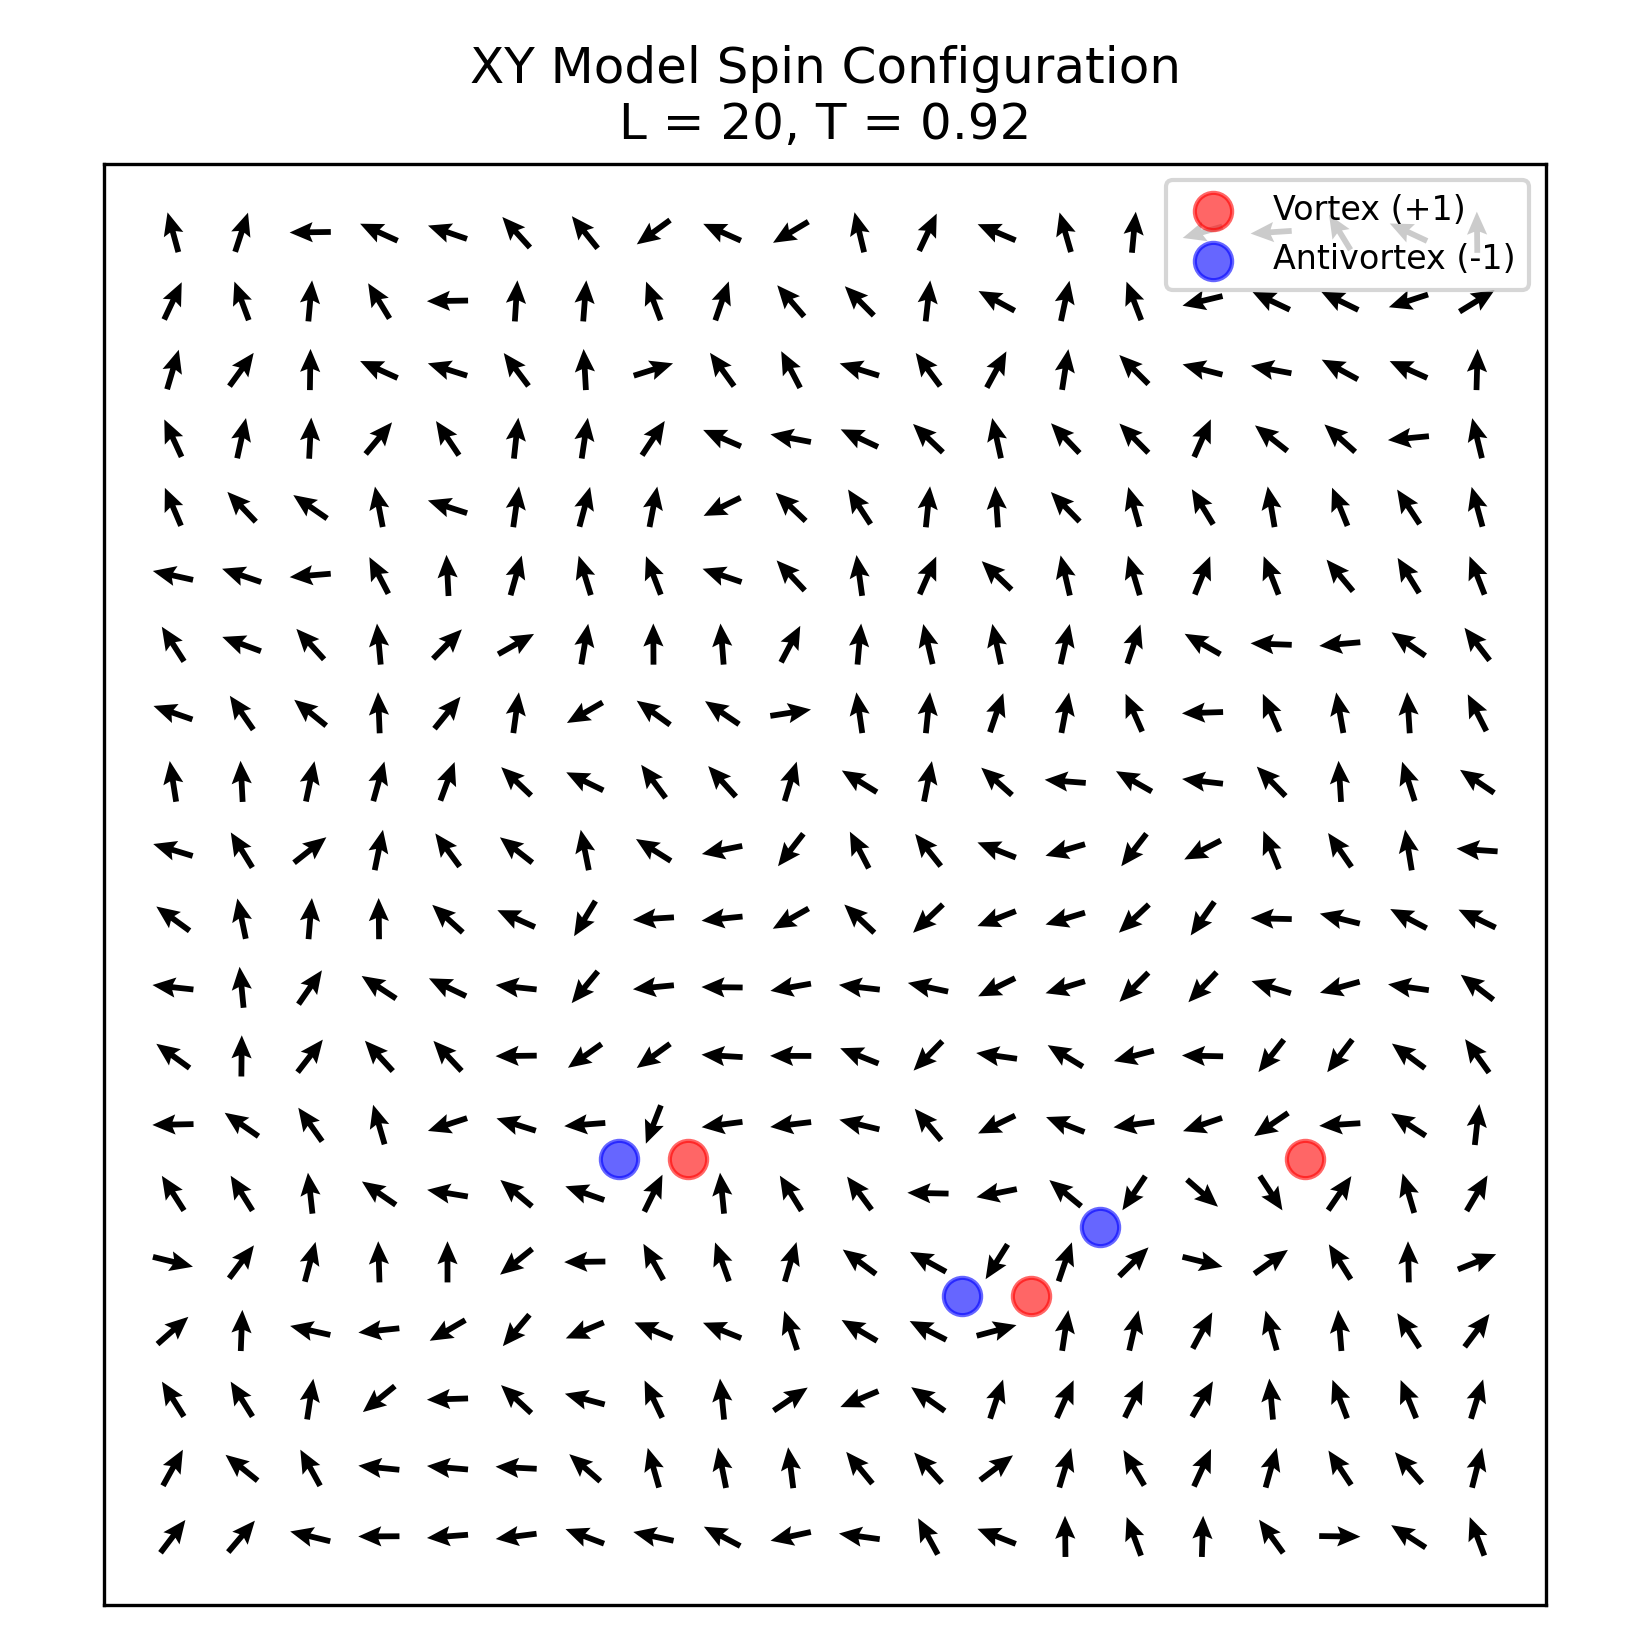
\includegraphics[width=\linewidth]{images/visualization/xy_model_L20_T0.92_vis.png}
            \tiny $T \approx 0.92 \gtrsim T_{KT}$\\(Pairs Unbinding)
        \end{column}
        \begin{column}{0.33\textwidth}
            \centering
            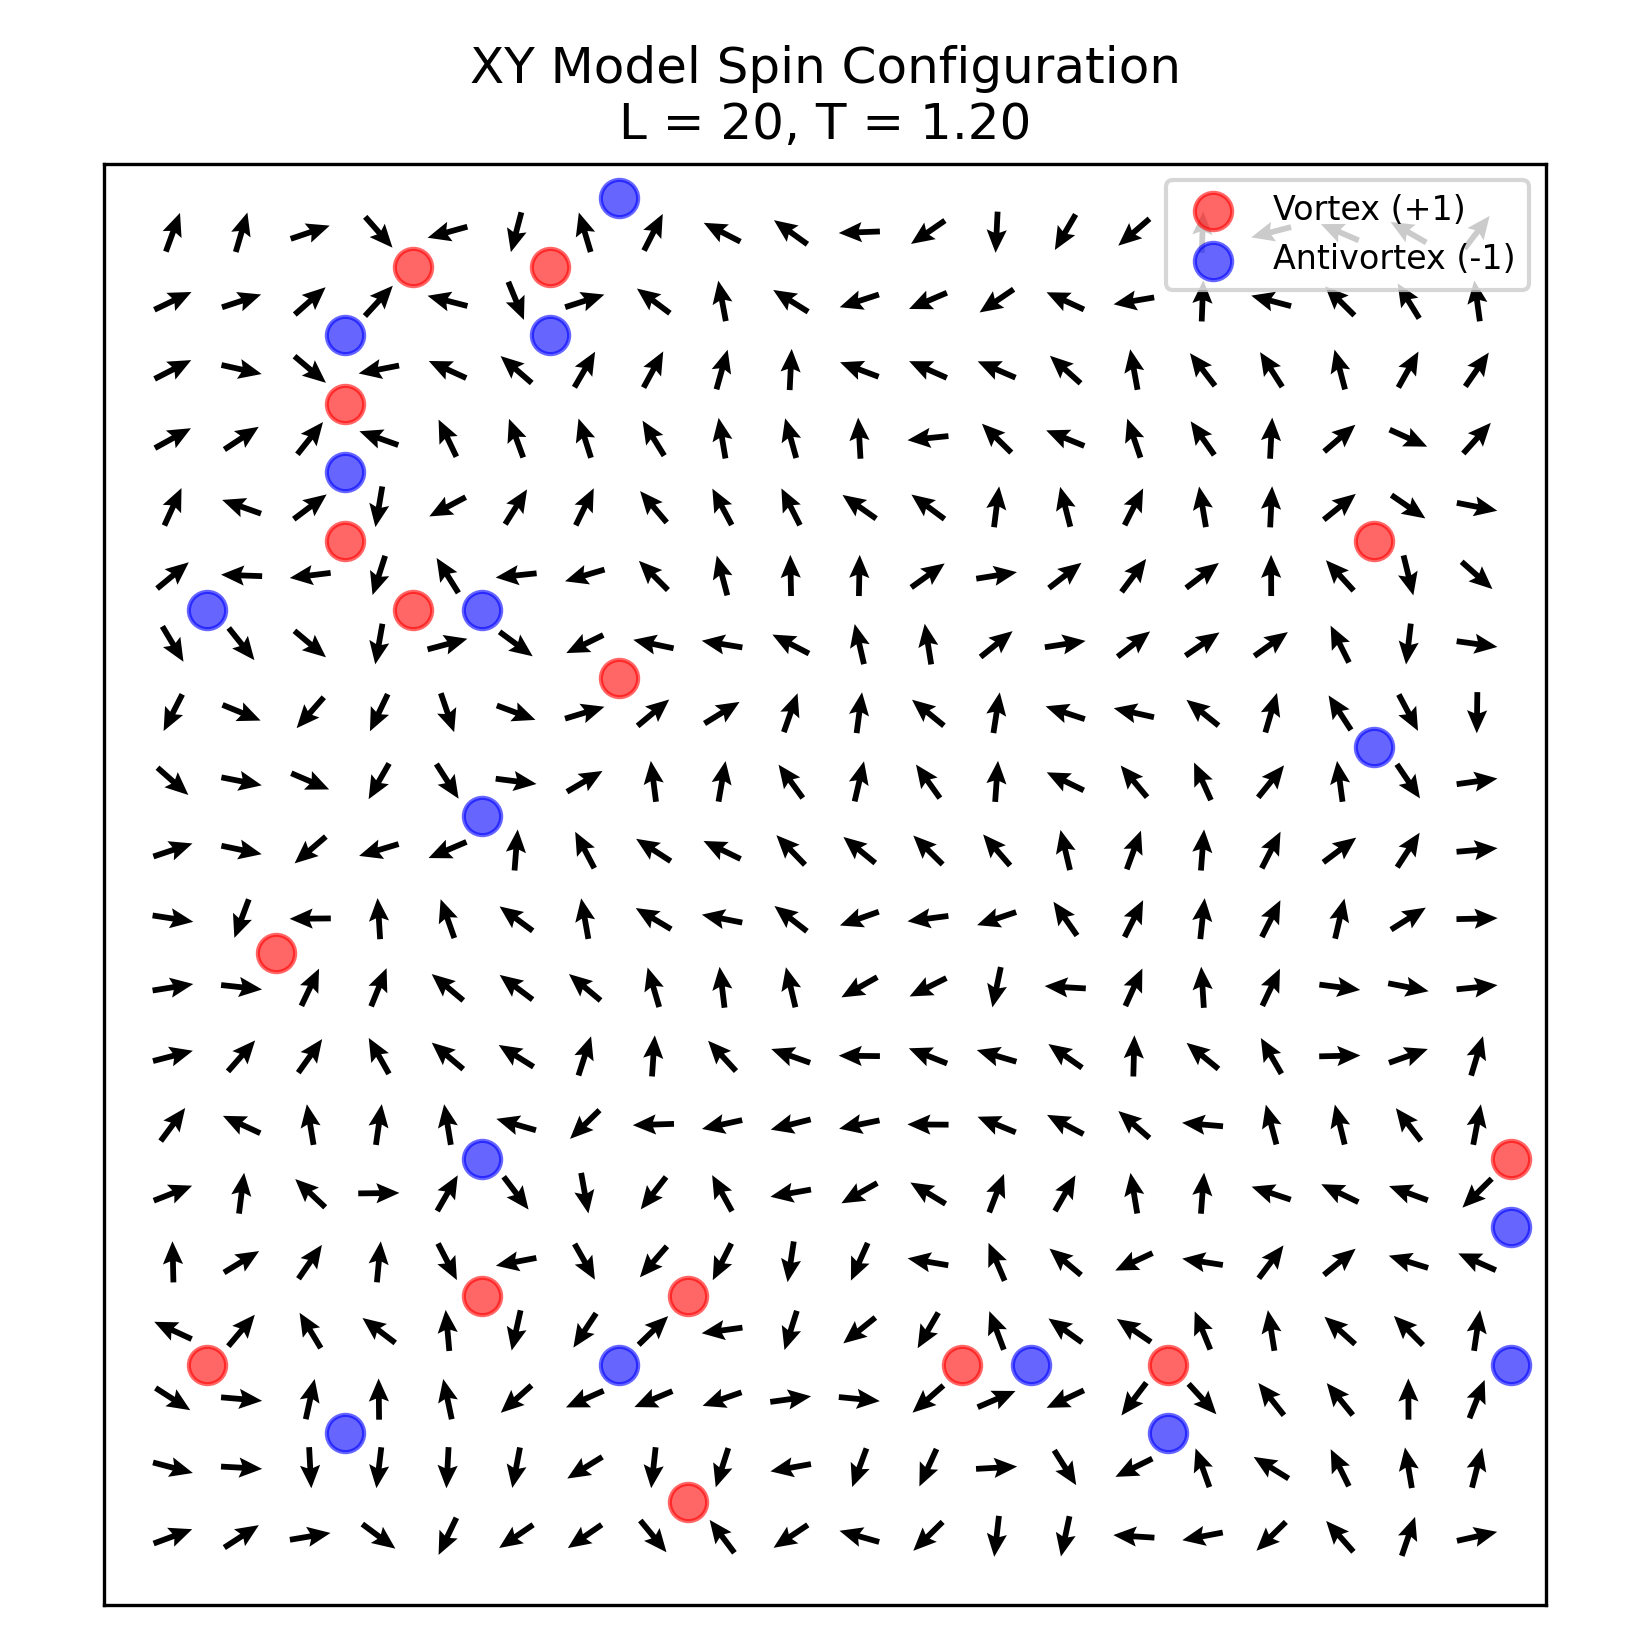
\includegraphics[width=\linewidth]{images/visualization/xy_model_L20_T1.20_vis.png}
            \tiny $T = 1.20 > T_{KT}$\\(Disordered, Free Vortices)
        \end{column}
    \end{columns}
    \vspace{0.5em}
    {\tiny Spin configurations for L=20 showing the transition from quasi-long-range order with bound vortex pairs (left) to a disordered state with proliferating free vortices (right). Red/Blue circles indicate vortex/antivortex locations.}
\end{frame}
% --- END NEW FRAME ---

\begin{frame}{Renormalization Group Analysis}
    \begin{itemize}
        \item Mapping to 2D Coulomb gas: vortices as charges with $\ln(r)$ interaction.
        \item Kosterlitz RG flow equations for effective coupling $K(l) = J_{\text{eff}}(l)/(k_B T)$ and vortex fugacity $y(l)$ at length scale $l$:
        \begin{align*}
            \frac{d K^{-1}(l)}{dl} &= 4 \pi^3 y(l)^2 + O(y(l)^4) \\
            \frac{d y(l)}{dl} &= (2 - \pi K(l)) y(l) + O(y(l)^3)
        \end{align*}
        \pause
        \item Flow diagram shows two phases separated by a line of fixed points:
        \begin{itemize}
            \item \textbf{Low-T} ($K > 2/\pi$): $y \to 0$ (vortices are irrelevant, QLRO prevails).
            \item \textbf{High-T} ($K < 2/\pi$): $y$ increases (vortices proliferate, destroying QLRO).
        \end{itemize}
    \end{itemize}
\end{frame}

\begin{frame}{Renormalization Group Analysis}
    \begin{itemize}
        \item Flow diagram shows two phases separated by a line of fixed points:
        \begin{itemize}
            \item \textbf{Low-T} ($K > 2/\pi$): $y \to 0$ (vortices are irrelevant, QLRO prevails).
            \item \textbf{High-T} ($K < 2/\pi$): $y$ increases (vortices proliferate, destroying QLRO).
        \end{itemize}
        \pause
        \item Universal predictions:
        \begin{itemize}
            \item Critical coupling: $K_c = 2/\pi \implies T_{KT} = \frac{\pi J}{2k_B}$.
            \item \textbf{Nelson-Kosterlitz jump}: Spin stiffness $\rho_s$ (helicity modulus) jumps discontinuously at the transition:
            \begin{equation*}
                \rho_s(T_{KT}^-) = \frac{2k_B T_{KT}}{\pi}
            \end{equation*}
            \item Correlation length above transition: $\xi(T) \sim \exp(b/\sqrt{T/T_{KT}-1})$.
        \end{itemize}
    \end{itemize}
\end{frame}

% --- Section 3: Monte Carlo Methods ---
\section{Monte Carlo Methods}

\begin{frame}{Simulating the XY Model}
    \begin{itemize}
        \item Challenges in simulating BKT transition:
            \begin{itemize}
                \item Critical slowing down near phase transition
                \item Need for large system sizes (finite-size effects)
                \item Long correlation times
            \end{itemize}
        \pause
        \item Standard Metropolis algorithm:
            \begin{itemize}
                \item Energy change for spin flip: $\Delta E = -J \sum_{\langle i,j \rangle} [\cos(\theta'_i - \theta_j) - \cos(\theta_i - \theta_j)]$
                \item Accept new state with probability $P = \min(1, e^{-\beta \Delta E})$
                \item Very inefficient near critical point due to large correlated regions
            \end{itemize}
        \pause
        \item More efficient approaches:
            \begin{itemize}
                \item \textbf{Wolff cluster algorithm (Implemented):} Updates entire clusters of spins, significantly reducing critical slowing down.
                \item \textit{Parallel tempering (Discussed):} Exchanges configurations between different temperatures to improve sampling (beneficial but not used in our final simulation code).
                % \item Combination of both methods for optimal efficiency
            \end{itemize}
    \end{itemize}
\end{frame}

\begin{frame}{Wolff Cluster Algorithm}
    \begin{itemize}
        \item Efficiently updates entire clusters of correlated spins
        \begin{enumerate}
            \item Choose a random reflection axis (unit vector $\mathbf{r}$)
            \item Pick a random initial site for the cluster
            \item Add neighboring spins with probability $P_{\text{add}} = 1 - \exp[\min(0, 2\beta J (\mathbf{S}_i \cdot \mathbf{r})(\mathbf{S}_j \cdot \mathbf{r}))]$
            \item Reflect all spins in the cluster w.r.t. the chosen axis
        \end{enumerate}
        \pause
        \item Advantages:
        \begin{itemize}
            \item Dramatically reduces critical slowing down
            \item Dynamical critical exponent $z \approx 0$ (vs. $z \approx 2$ for Metropolis)
            \item Efficiently samples low-energy configurations
        \end{itemize}
        \pause
        \item Our implementation (`simulate.py`):
        \begin{itemize}
            % \item Combines Wolff updates with parallel tempering
            % \item Optimally adapts the number of updates based on average cluster size
            \item Uses the Wolff algorithm (or Metropolis as an option).
            \item Leverages Numba JIT compilation for performance.
            \item Runs simulations for different temperatures in parallel using multiprocessing.
            \item \textit{Note: Does not implement Parallel Tempering (Replica Exchange).}
        \end{itemize}
    \end{itemize}
\end{frame}

\begin{frame}{Parallel Tempering}
    \begin{itemize}
        \item \textit{(Method discussed for context, not implemented in `simulate.py` results)}
        \item Simulates multiple replicas at different temperatures $T_1 < T_2 < ... < T_M$
        \item Periodically proposes exchanges between adjacent temperatures
        \begin{itemize}
            \item Accept exchange with probability $P = \min(1, \exp((\beta_i - \beta_j)(E_j - E_i)))$
        \end{itemize}
        \pause
        \item Benefits:
        \begin{itemize}
            \item Helps systems escape from local minima
            \item Improves sampling at low temperatures
            \item Configurations can diffuse across temperature space
        \end{itemize}
        \pause
        \item Implementation details (if used):
        \begin{itemize}
            \item Alternating even/odd exchanges for better mixing
            \item Temperature spacing optimized for exchange acceptance rates
            \item Often combined with cluster algorithms like Wolff for optimal efficiency
        \end{itemize}
    \end{itemize}
\end{frame}

% --- Section 4: Implementation ---
\section{Implementation Details}

\begin{frame}{Our Implementation Approach}
    \begin{itemize}
        \item Simulation structure:
        \begin{enumerate}
            \item \textbf{Initial Equilibration}: Run sufficient updates to forget initial state.
            \item \textbf{Thermalization}: Ensure equilibrium is reached at each target temperature (often combined with equilibration).
            \item \textbf{Measurement}: Collect statistics over long runs in equilibrium.
        \end{enumerate}
        \pause
        \item Optimization techniques:
        \begin{itemize}
            \item Numba `@njit` compilation for core simulation loops (Wolff update, energy calculation).
            \item Vectorized operations with NumPy where possible.
            \item Pre-computation of neighbor indices.
            %\item (Optional: Dynamic adjustment of updates per sweep based on avg. cluster size / acceptance rates).
        \end{itemize}
        \pause
        \item Simulation workflow:
        \begin{itemize}
            \item Define temperature range and system sizes $L$.
            \item Run independent simulations for each $(L, T)$ using Wolff algorithm (and potentially Parallel Tempering).
            \item Thermalize, then collect measurements (Energy, Stiffness, etc.) over many sweeps.
            \item Calculate averages and estimate errors (e.g., via Jackknife).
            \item Perform finite-size scaling analysis to extract $T_{KT}$ and critical exponents.
        \end{itemize}
    \end{itemize}
\end{frame}

\begin{frame}{Key Observables}
    \begin{itemize}
        \item Physical quantities measured in our simulation:
        \begin{itemize}
            \item \textbf{Energy per spin}: $e = \frac{\langle H \rangle}{N} = -\frac{J}{N} \sum_{\langle i,j \rangle} \langle\cos(\theta_i - \theta_j)\rangle$
            \item \textbf{Specific heat}: $c_v = \frac{\langle E^2 \rangle - \langle E \rangle^2}{NT^2}$
            \item \textbf{Magnetization}: $\mathbf{m} = \frac{1}{N}\left\langle \sum_i (\cos\theta_i, \sin\theta_i) \right\rangle$
            \item \textbf{Susceptibility}: $\chi = \frac{\langle M^2 \rangle - \langle M \rangle^2}{NT}$
            \pause
            \item \textbf{Spin stiffness (Helicity modulus)}:
            \begin{equation*}
                \rho_s = \langle H_x \rangle - \frac{\beta}{N} \langle I_x^2 \rangle
            \end{equation*}
            where $H_x = \sum_{\langle i,j \rangle_x} \cos(\theta_i - \theta_j)$ and $I_x = \sum_{\langle i,j \rangle_x} \sin(\theta_i - \theta_j)$
            \pause
            \item \textbf{Vortex density}: $\omega_v = \frac{1}{N} \sum_{\text{plaquettes}} \left| \frac{1}{2\pi} \sum_{\text{edges}} \Delta\theta_{ij} \right|$
        \end{itemize}
        \item Spin stiffness is crucial for locating $T_{KT}$ through the universal jump
    \end{itemize}
\end{frame}

\begin{frame}{Error Analysis}
    \begin{itemize}
        \item Statistical errors from Monte Carlo sampling:
        \begin{itemize}
            \item Sequential MC data is \textit{correlated}
            \item Standard error formulas for independent data are inadequate
        \end{itemize}
        \pause
        \item Jackknife resampling for reliable error estimation:
        \begin{enumerate}
            \item Divide data into $B$ blocks larger than correlation time
            \item For each block $b$, compute estimate $\bar{O}_b$ by excluding block $b$
            \item Jackknife error: $\sigma^2_{\text{JK}} = \frac{B-1}{B}\sum_b (\bar{O}_b - \bar{O})^2$
        \end{enumerate}
        \pause
        \item Benefits:
        \begin{itemize}
            \item Correctly accounts for autocorrelations in MC data
            \item Works well for derived quantities (non-linear functions)
            \item More reliable than naive variance calculations
            \item Essential for accurate error bars on quantities near transition
        \end{itemize}
    \end{itemize}
\end{frame}

% --- Section 5: Results and Analysis ---
\section{Results and Analysis}

\begin{frame}{Energy and Specific Heat}

    % First pair: Energy text and image
    \begin{columns}[T] % Align tops
        \begin{column}{0.5\textwidth}
            \textbf{Internal Energy per Spin ($e$)}
            \begin{itemize}
                \item Smoothly decreases with temperature.
                \item Weak dependence on system size $L$.
                \item No sharp features indicating the transition.
            \end{itemize}
        \end{column}
        \begin{column}{0.5\textwidth}
            
\includegraphics[width=0.65\linewidth]{images/observables/xy_model_energy_wolff.png}
        \end{column}
    \end{columns}

    \vspace{1em} % Adjust vertical space between pairs as needed

    % Second pair: Specific Heat text and image
    \begin{columns}[T] % Align tops
        \begin{column}{0.5\textwidth}
            \textbf{Specific Heat ($c_v$)}
            \begin{itemize}
                \item Exhibits a broad peak around $T \approx 1.0 J$.
                \item Peak height increases slightly with $L$.
                \item \mathalert{Crucially, no divergence} at $T_{KT}$, consistent with infinite-order BKT transition.
            \end{itemize}
        \end{column}
        \begin{column}{0.5\textwidth}
            
\includegraphics[width=0.65\linewidth]{images/observables/xy_model_specific_heat_wolff.png}
        \end{column}
    \end{columns}

\end{frame}

\begin{frame}{Magnetization and Susceptibility}

    % First pair: Magnetization text and image
    \begin{columns}[T] % Align tops
        \begin{column}{0.5\textwidth}
            \textbf{Magnetization ($|\mathbf{m}|$)}
            \begin{itemize}
                \item Suppressed at finite $T$ for finite $L$, consistent with Mermin-Wagner.
                \item Slow decay with $L$ in the low-T phase, compatible with algebraic decay ($|\mathbf{m}| \sim L^{-\eta(T)/2}$) expected for QLRO.
                \item Faster decay in the high-T phase.
            \end{itemize}
        \end{column}
        \begin{column}{0.5\textwidth}
             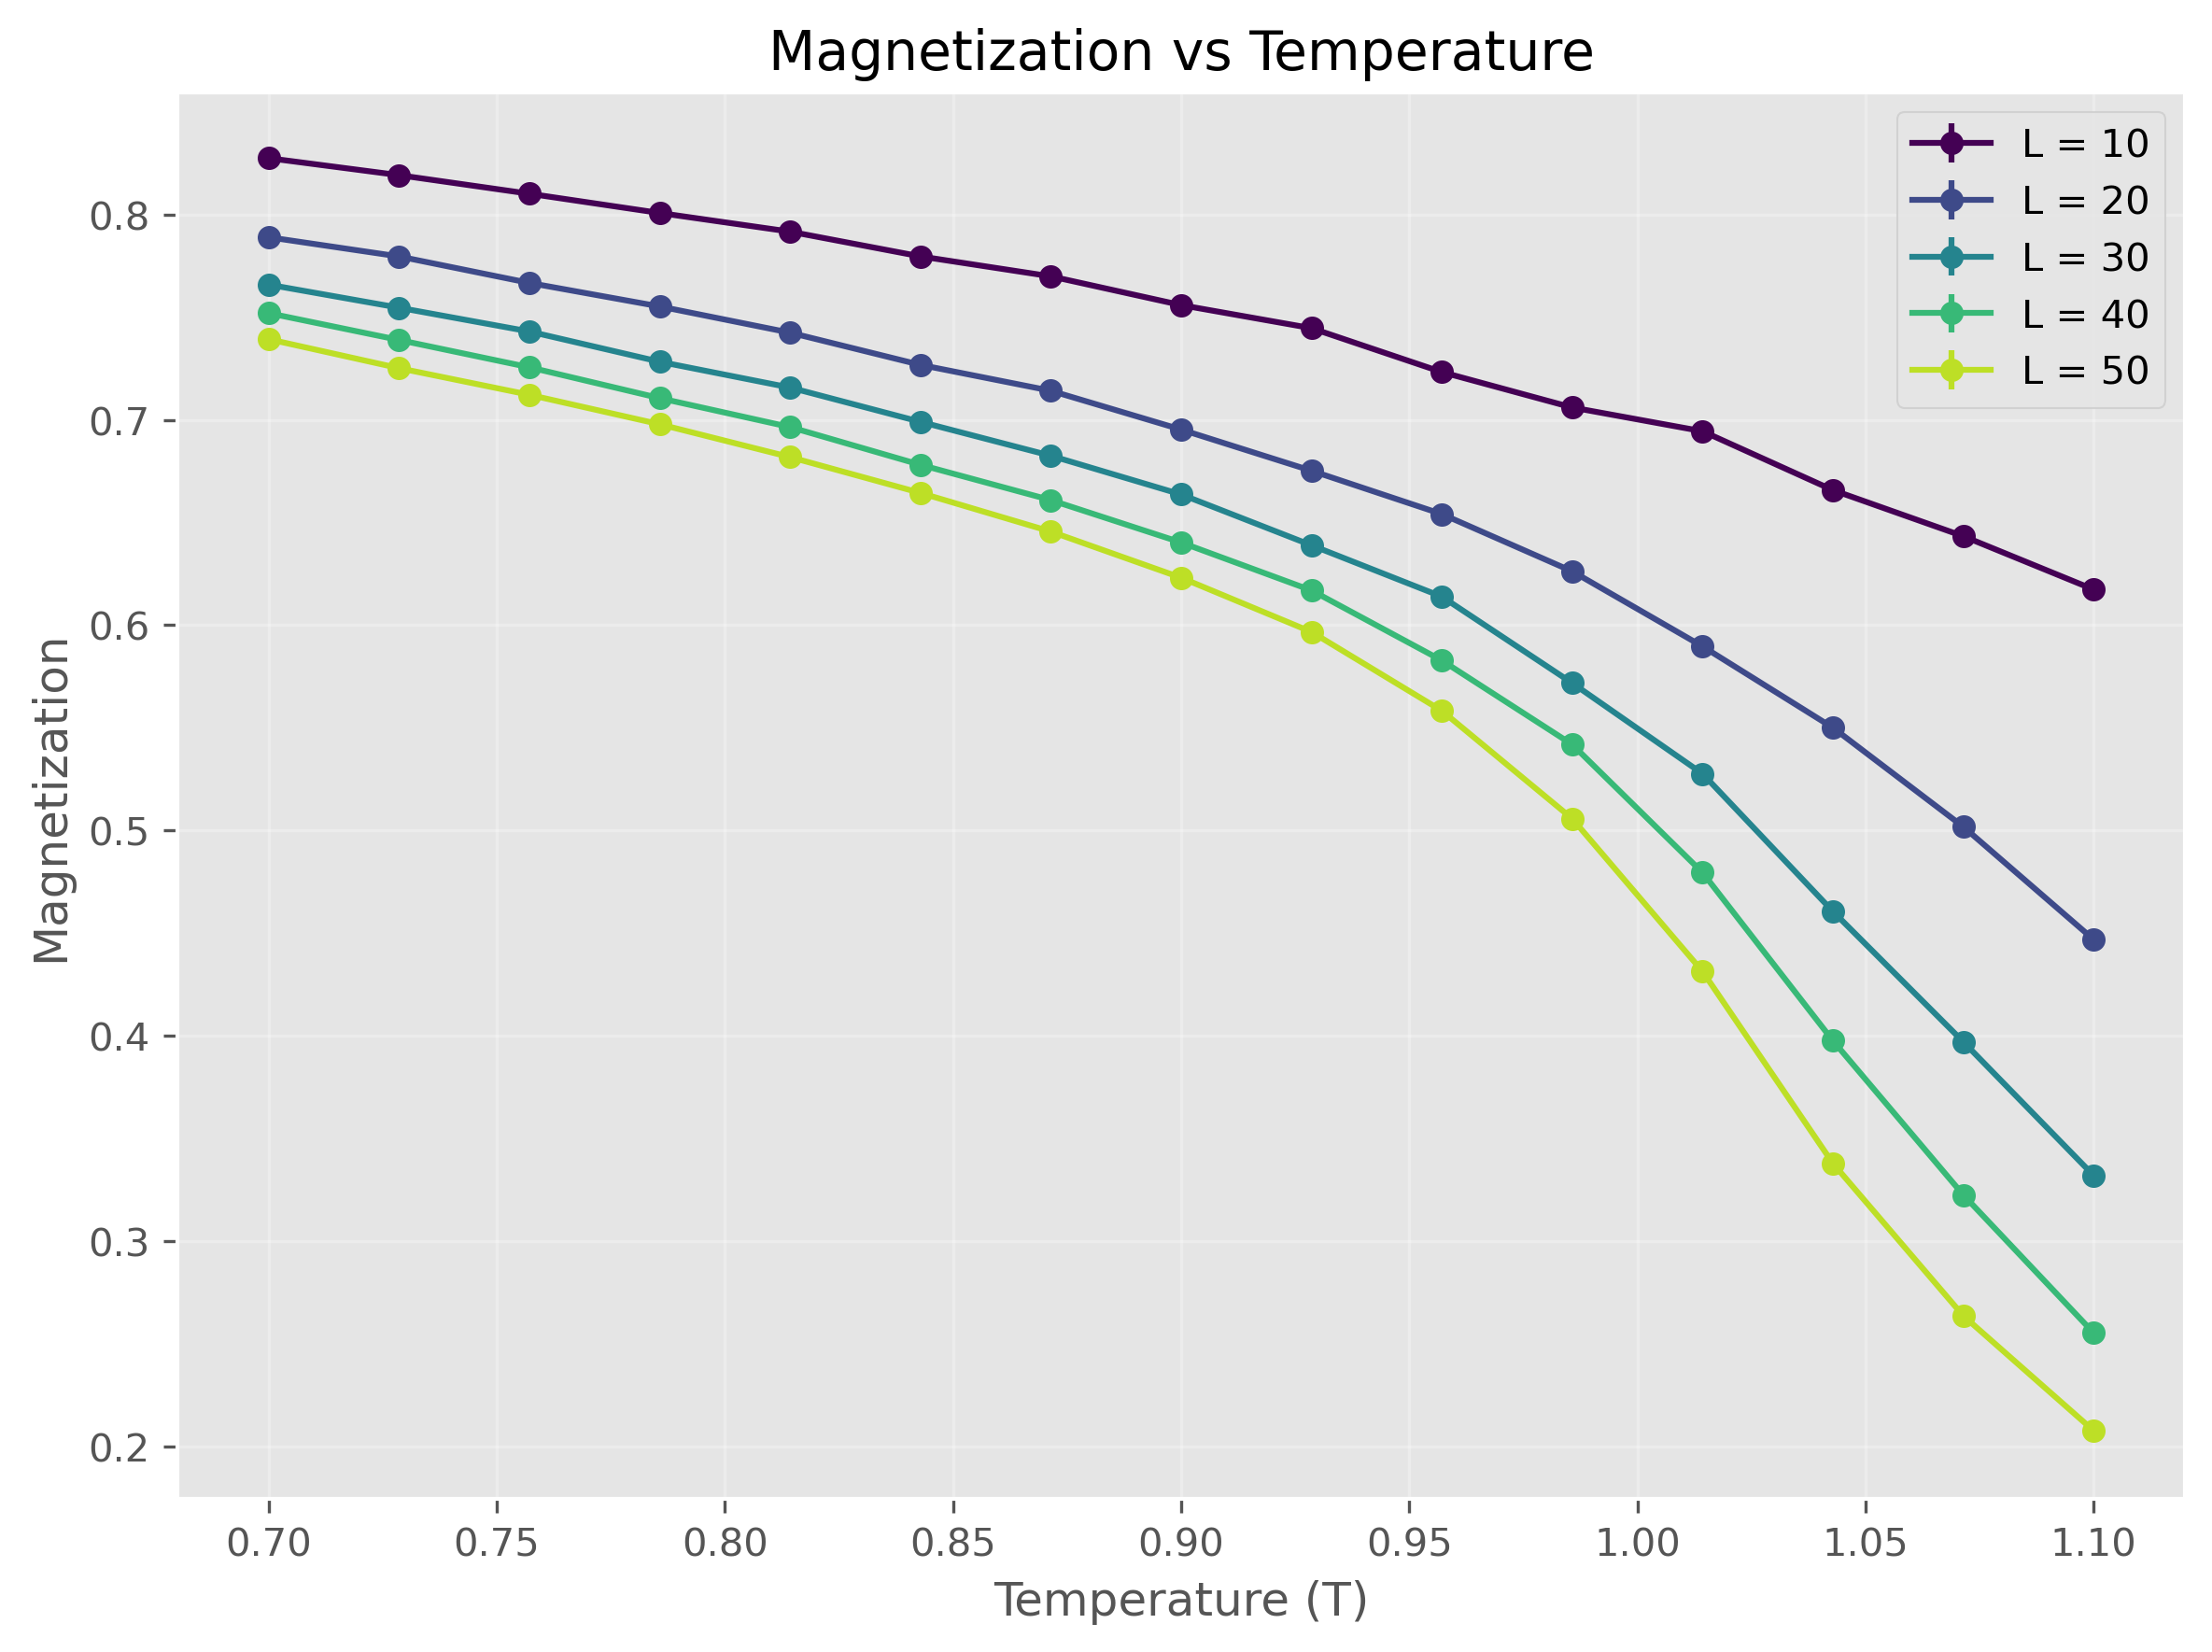
\includegraphics[width=0.65\linewidth]{images/observables/xy_model_magnetization_wolff.png}
        \end{column}
    \end{columns}

    \vspace{1em} % Adjust vertical space between pairs as needed

    % Second pair: Susceptibility text and image
    \begin{columns}[T] % Align tops
        \begin{column}{0.5\textwidth}
            \textbf{Susceptibility ($\chi$)}
            \begin{itemize}
                \item Develops a peak near the transition region.
                \item Peak height grows significantly with $L$.
                \item Diverges as $L \to \infty$ for $T \le T_{KT}$.
                \item Provides an alternative route to estimate $T_{KT}$, though less precise than stiffness.
            \end{itemize}
        \end{column}
        \begin{column}{0.5\textwidth}
             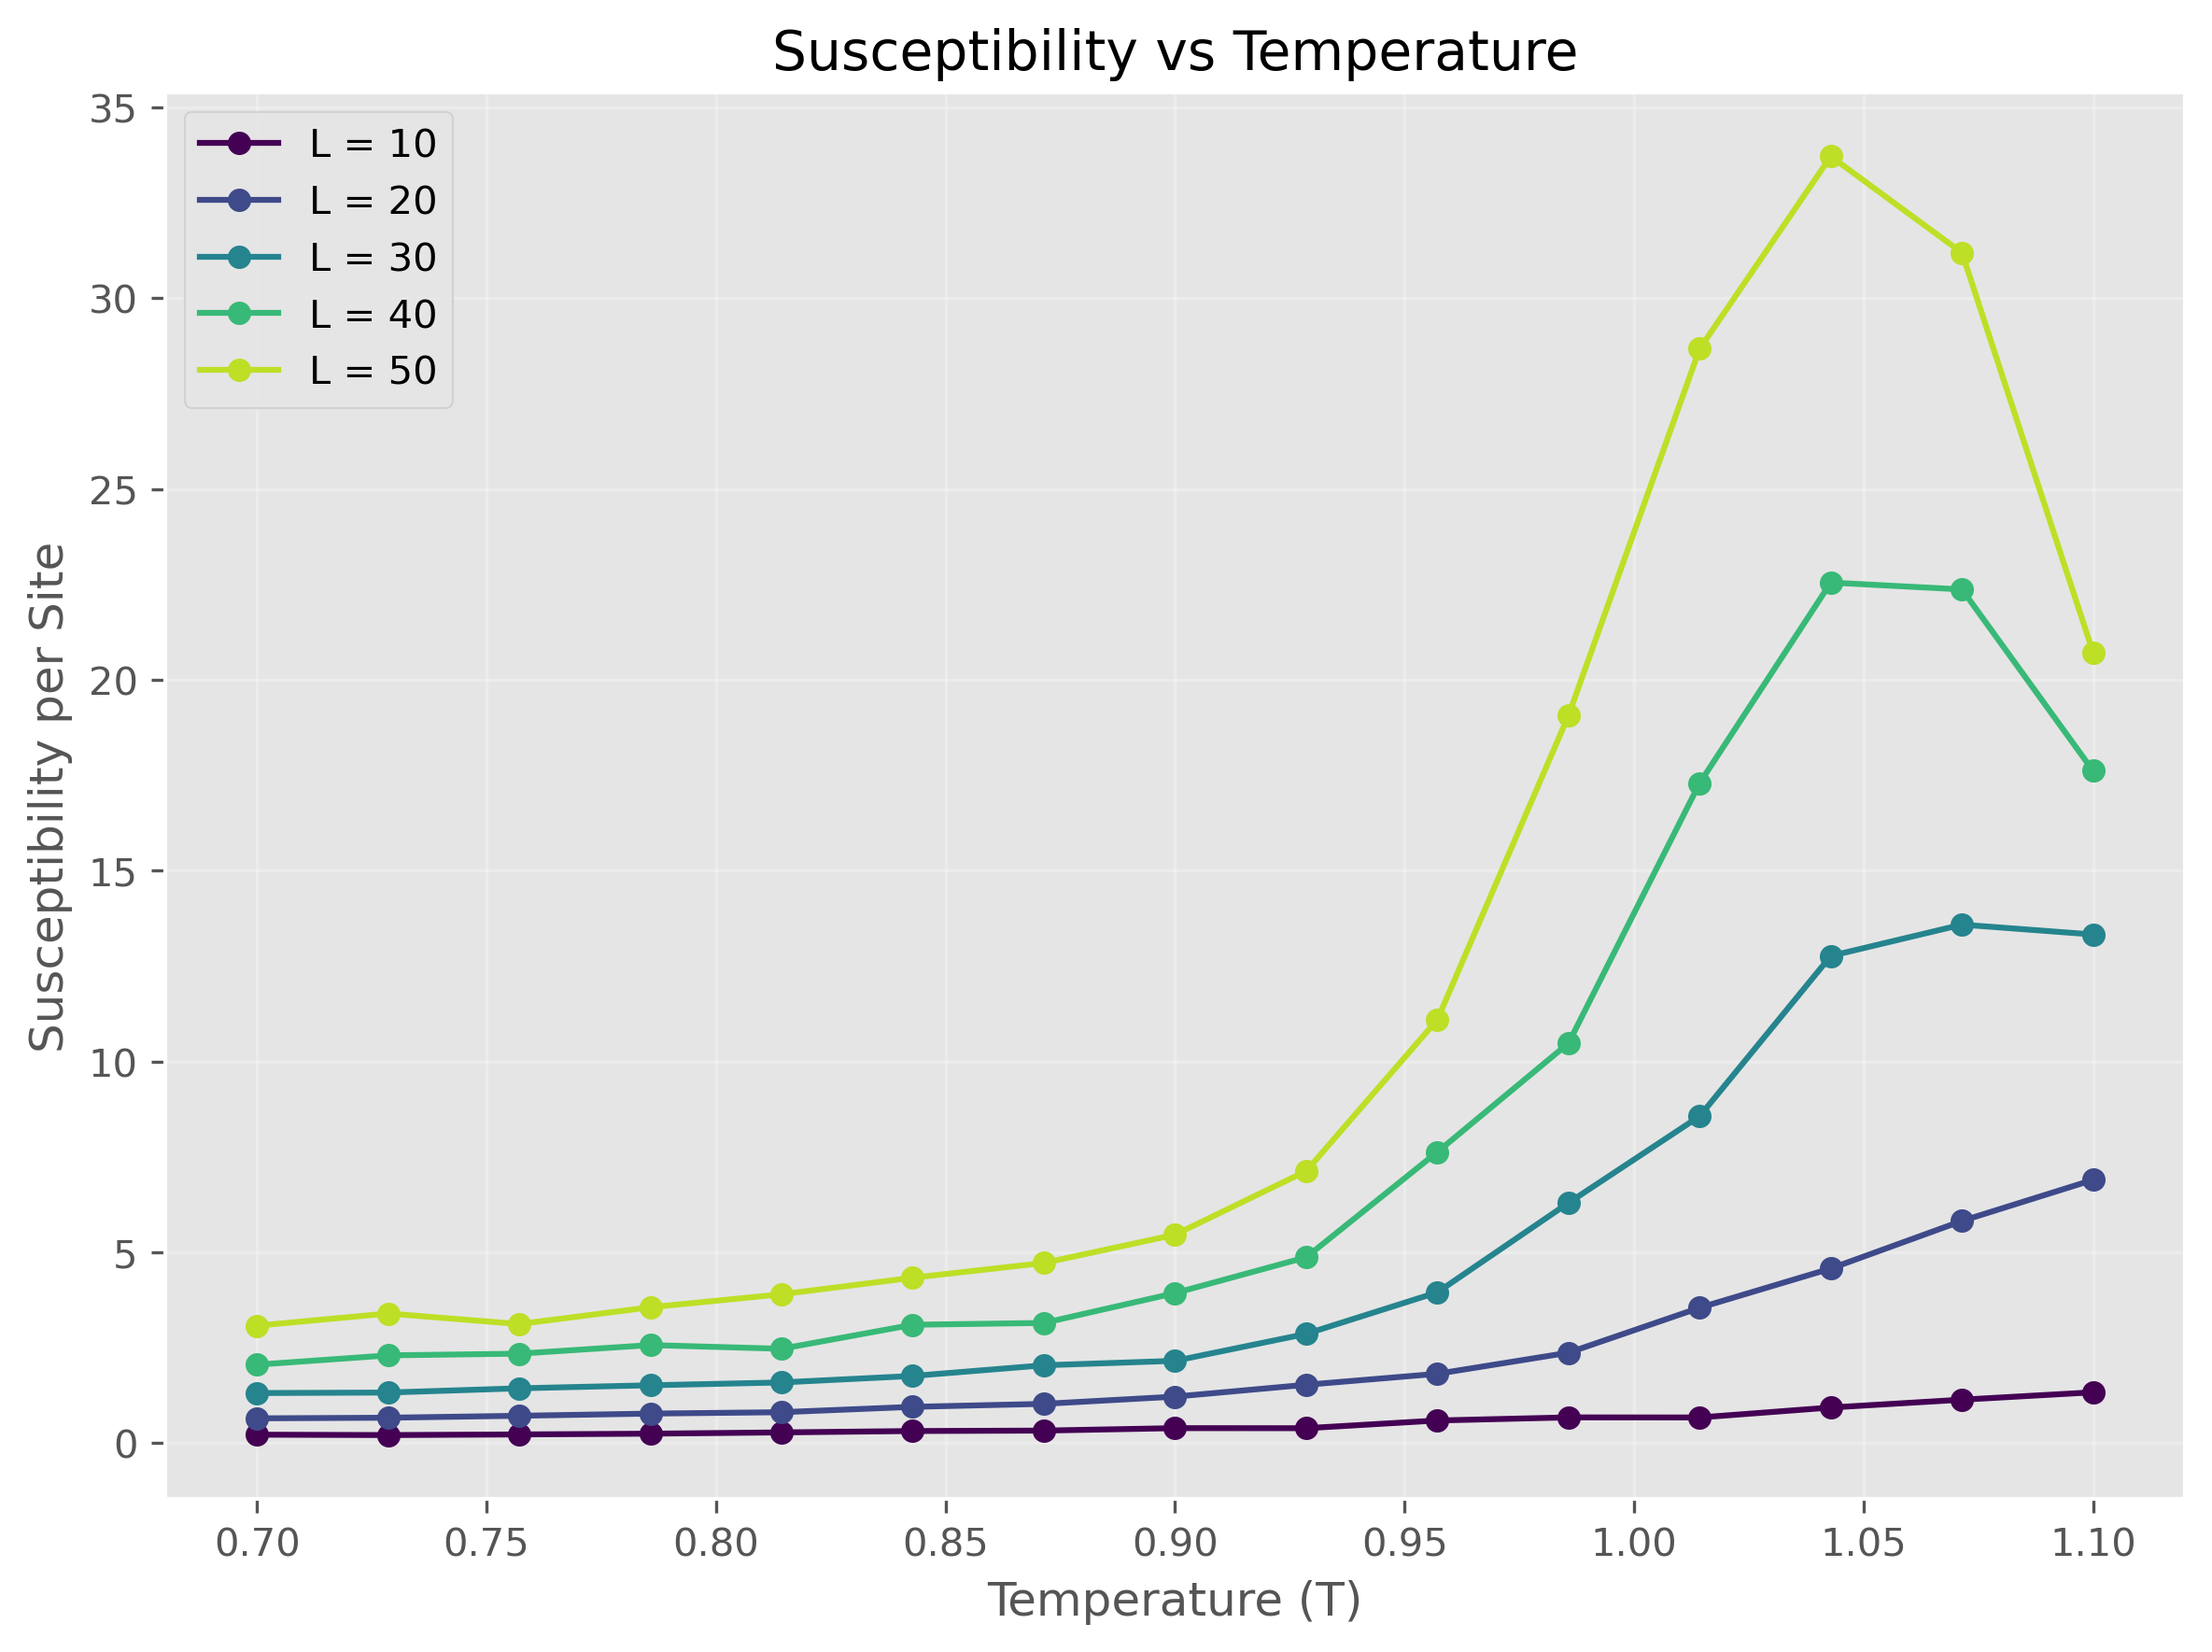
\includegraphics[width=0.65\linewidth]{images/observables/xy_model_susceptibility_wolff.png}
        \end{column}
    \end{columns}

\end{frame}





\begin{frame}{Binder Cumulant}

    % First pair: Binder cumulant text and image
    \begin{columns}[T] % Align tops
        \begin{column}{0.5\textwidth}
            \textbf{Binder Cumulant ($|\mathbf{U_L}|$)}
            \begin{itemize}
                \item ...
            \end{itemize}
        \end{column}
        \begin{column}{0.5\textwidth}
             
\includegraphics[width=0.65\linewidth]{images/observables/xy_model_binder_cumulant_wolff.png}
        \end{column}
    \end{columns}

    \vspace{1em} % Adjust vertical space between pairs as needed

    

\end{frame}












\begin{frame}{Spin Stiffness (Helicity Modulus $\rho_s$)}
    \begin{columns}[T]
        \begin{column}{0.55\textwidth}
            \textbf{Identifying the BKT Transition}
             \begin{itemize}
                \item Spin stiffness measures the free energy cost of applying a small twist to the boundary conditions.
                \item Decreases monotonically with temperature.
                \item \mathalert{Key indicator}: Universal jump prediction by Nelson-Kosterlitz:
                \\[0.5em] % Add space before equation
                $\qquad \rho_s(T_{KT}^-) = \frac{2 k_B T_{KT}}{\pi}$
                \\[0.5em] % Add space after equation
                \item Finite-size systems show smooth curves crossing the universal line $y = 2k_B T/\pi$.
                \item Intersection of $\rho_s(T, L)$ with this line provides a size-dependent estimate $T_{KT}(L)$.
                \item The convergence point of these intersections for $L \to \infty$ yields $T_{KT}(\infty)$.
                \item Our data suggests $T_{KT} \approx 0.89 J/k_B$.
            \end{itemize}
        \end{column}
        \begin{column}{0.45\textwidth}
            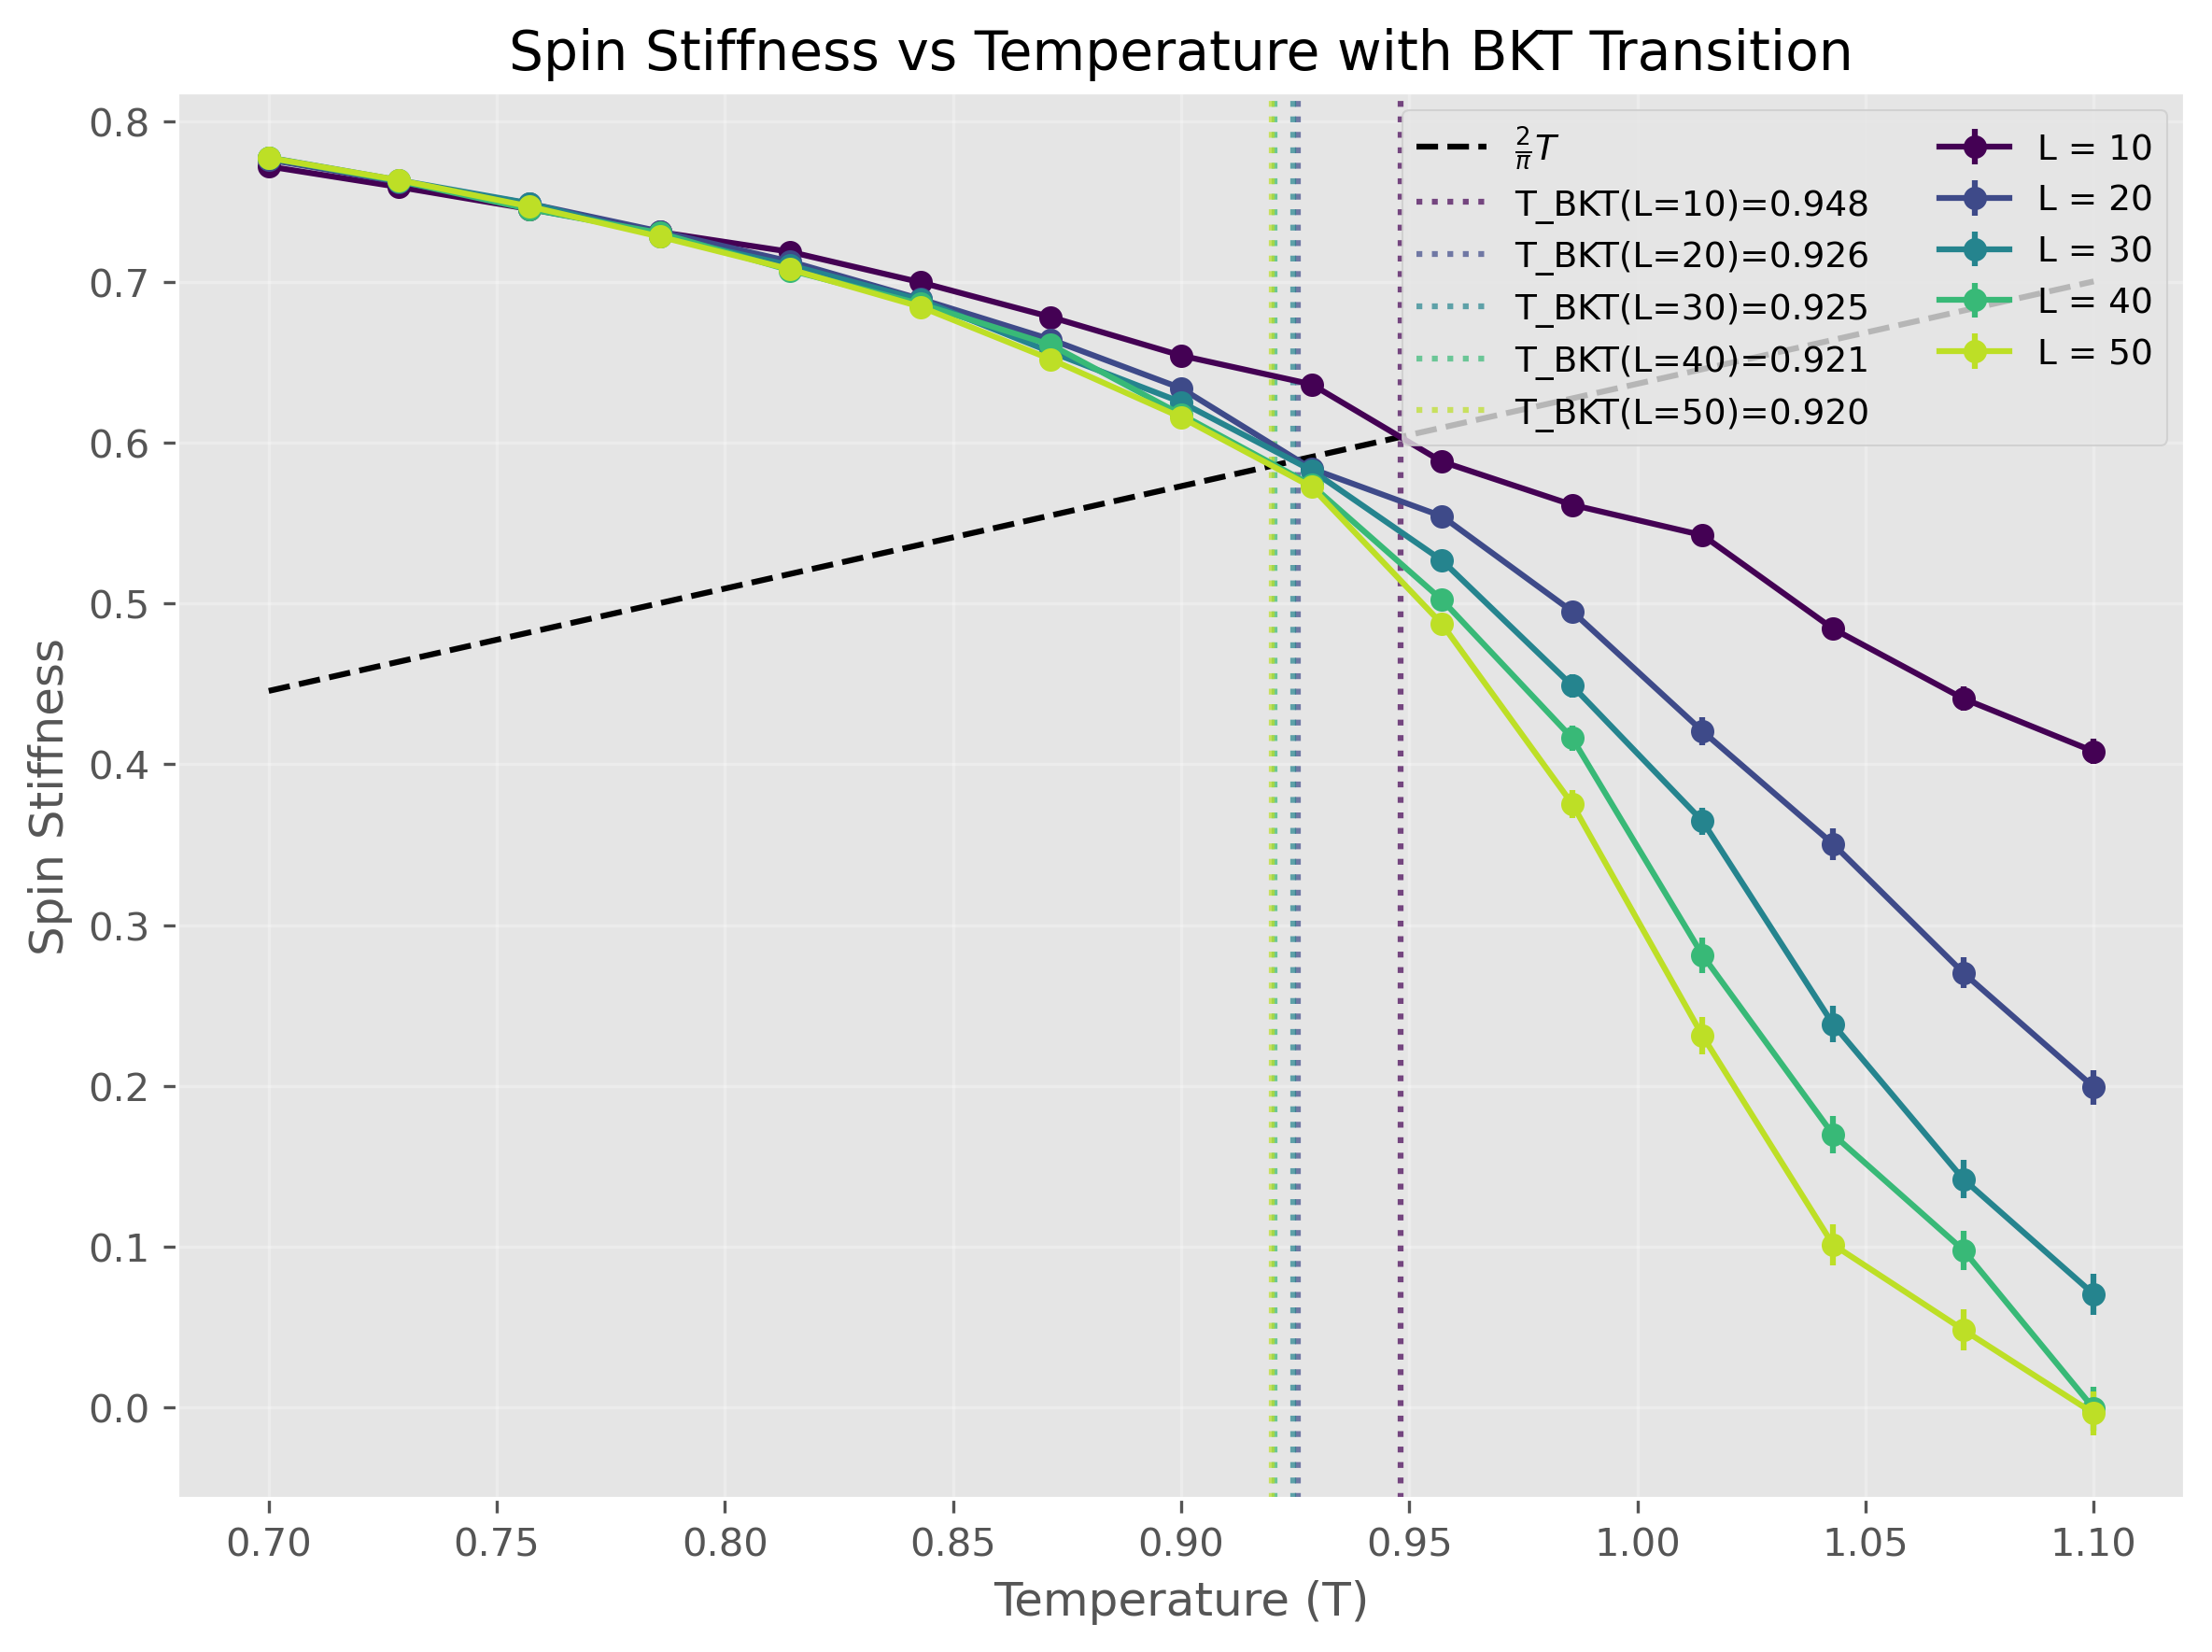
\includegraphics[width=\linewidth]{images/observables/xy_model_stiffness_wolff.png}
            \vspace{0.5em}
            {\tiny Plot shows $\rho_s$ vs $T$ for different $L$. Dashed line: $y = 2k_B T/\pi$.}
        \end{column}
    \end{columns}
\end{frame}




\begin{frame}{Decay exponent ($\eta$)}
    \begin{columns}[T]
        \begin{column}{0.55\textwidth}
            \textbf{Identifying the BKT Transition}
             \begin{itemize}
                \item 
                
            \end{itemize}
        \end{column}
        \begin{column}{0.45\textwidth}
            
\includegraphics[width=\linewidth]{images/observables/xy_model_eta_wolff.png}
            \vspace{0.5em}
            {\tiny Plot shows $\eta$ vs $T$ for different $L$. Dashed line: $y = 0.25$.}
        \end{column}
    \end{columns}
\end{frame}

\begin{frame}{Correlation length ($\xi$)}
    \begin{columns}[T]
        \begin{column}{0.55\textwidth}
             \begin{itemize}
                \item 
                
            \end{itemize}
        \end{column}
        \begin{column}{0.45\textwidth}
            
\includegraphics[width=\linewidth]{images/observables/xy_model_xi_wolff.png}
            \vspace{0.5em}
            {\tiny Plot shows $\xi$ vs $T$ for different $L$.}
        \end{column}
    \end{columns}
\end{frame}




\begin{frame}{Vortex Density}
    \begin{columns}[T]
        \begin{column}{0.55\textwidth}
            \textbf{Role of Topological Defects}
            \begin{itemize} % Consider adding [nosep] or [itemsep=0pt] here if needed (requires enumitem package)
                \item Vortex density $\omega_v$ measures the concentration of topological defects.
                \item At low temperatures ($T \ll T_{KT}$):
                    \begin{itemize} % Consider adding [nosep] or [itemsep=0pt] here
                        \item Vortices exist only in tightly bound vortex-antivortex pairs.
                        \item Measured density is very low.
                    \end{itemize}
                \item Near $T_{KT}$:
                    \begin{itemize} % Consider adding [nosep] or [itemsep=0pt] here
                        \item Pairs start to unbind.
                        \item Density increases sharply.
                    \end{itemize}
                \item Above $T_{KT}$:
                    \begin{itemize} % Consider adding [nosep] or [itemsep=0pt] here
                        \item Proliferation of free vortices/antivortices.
                        \item Density becomes significant, screening interactions and destroying QLRO.
                    \end{itemize}
                 \item Microscopic view of the transition mechanism.
            \end{itemize}
        \end{column}
        \begin{column}{0.45\textwidth}
            % Reduce image width from \linewidth
            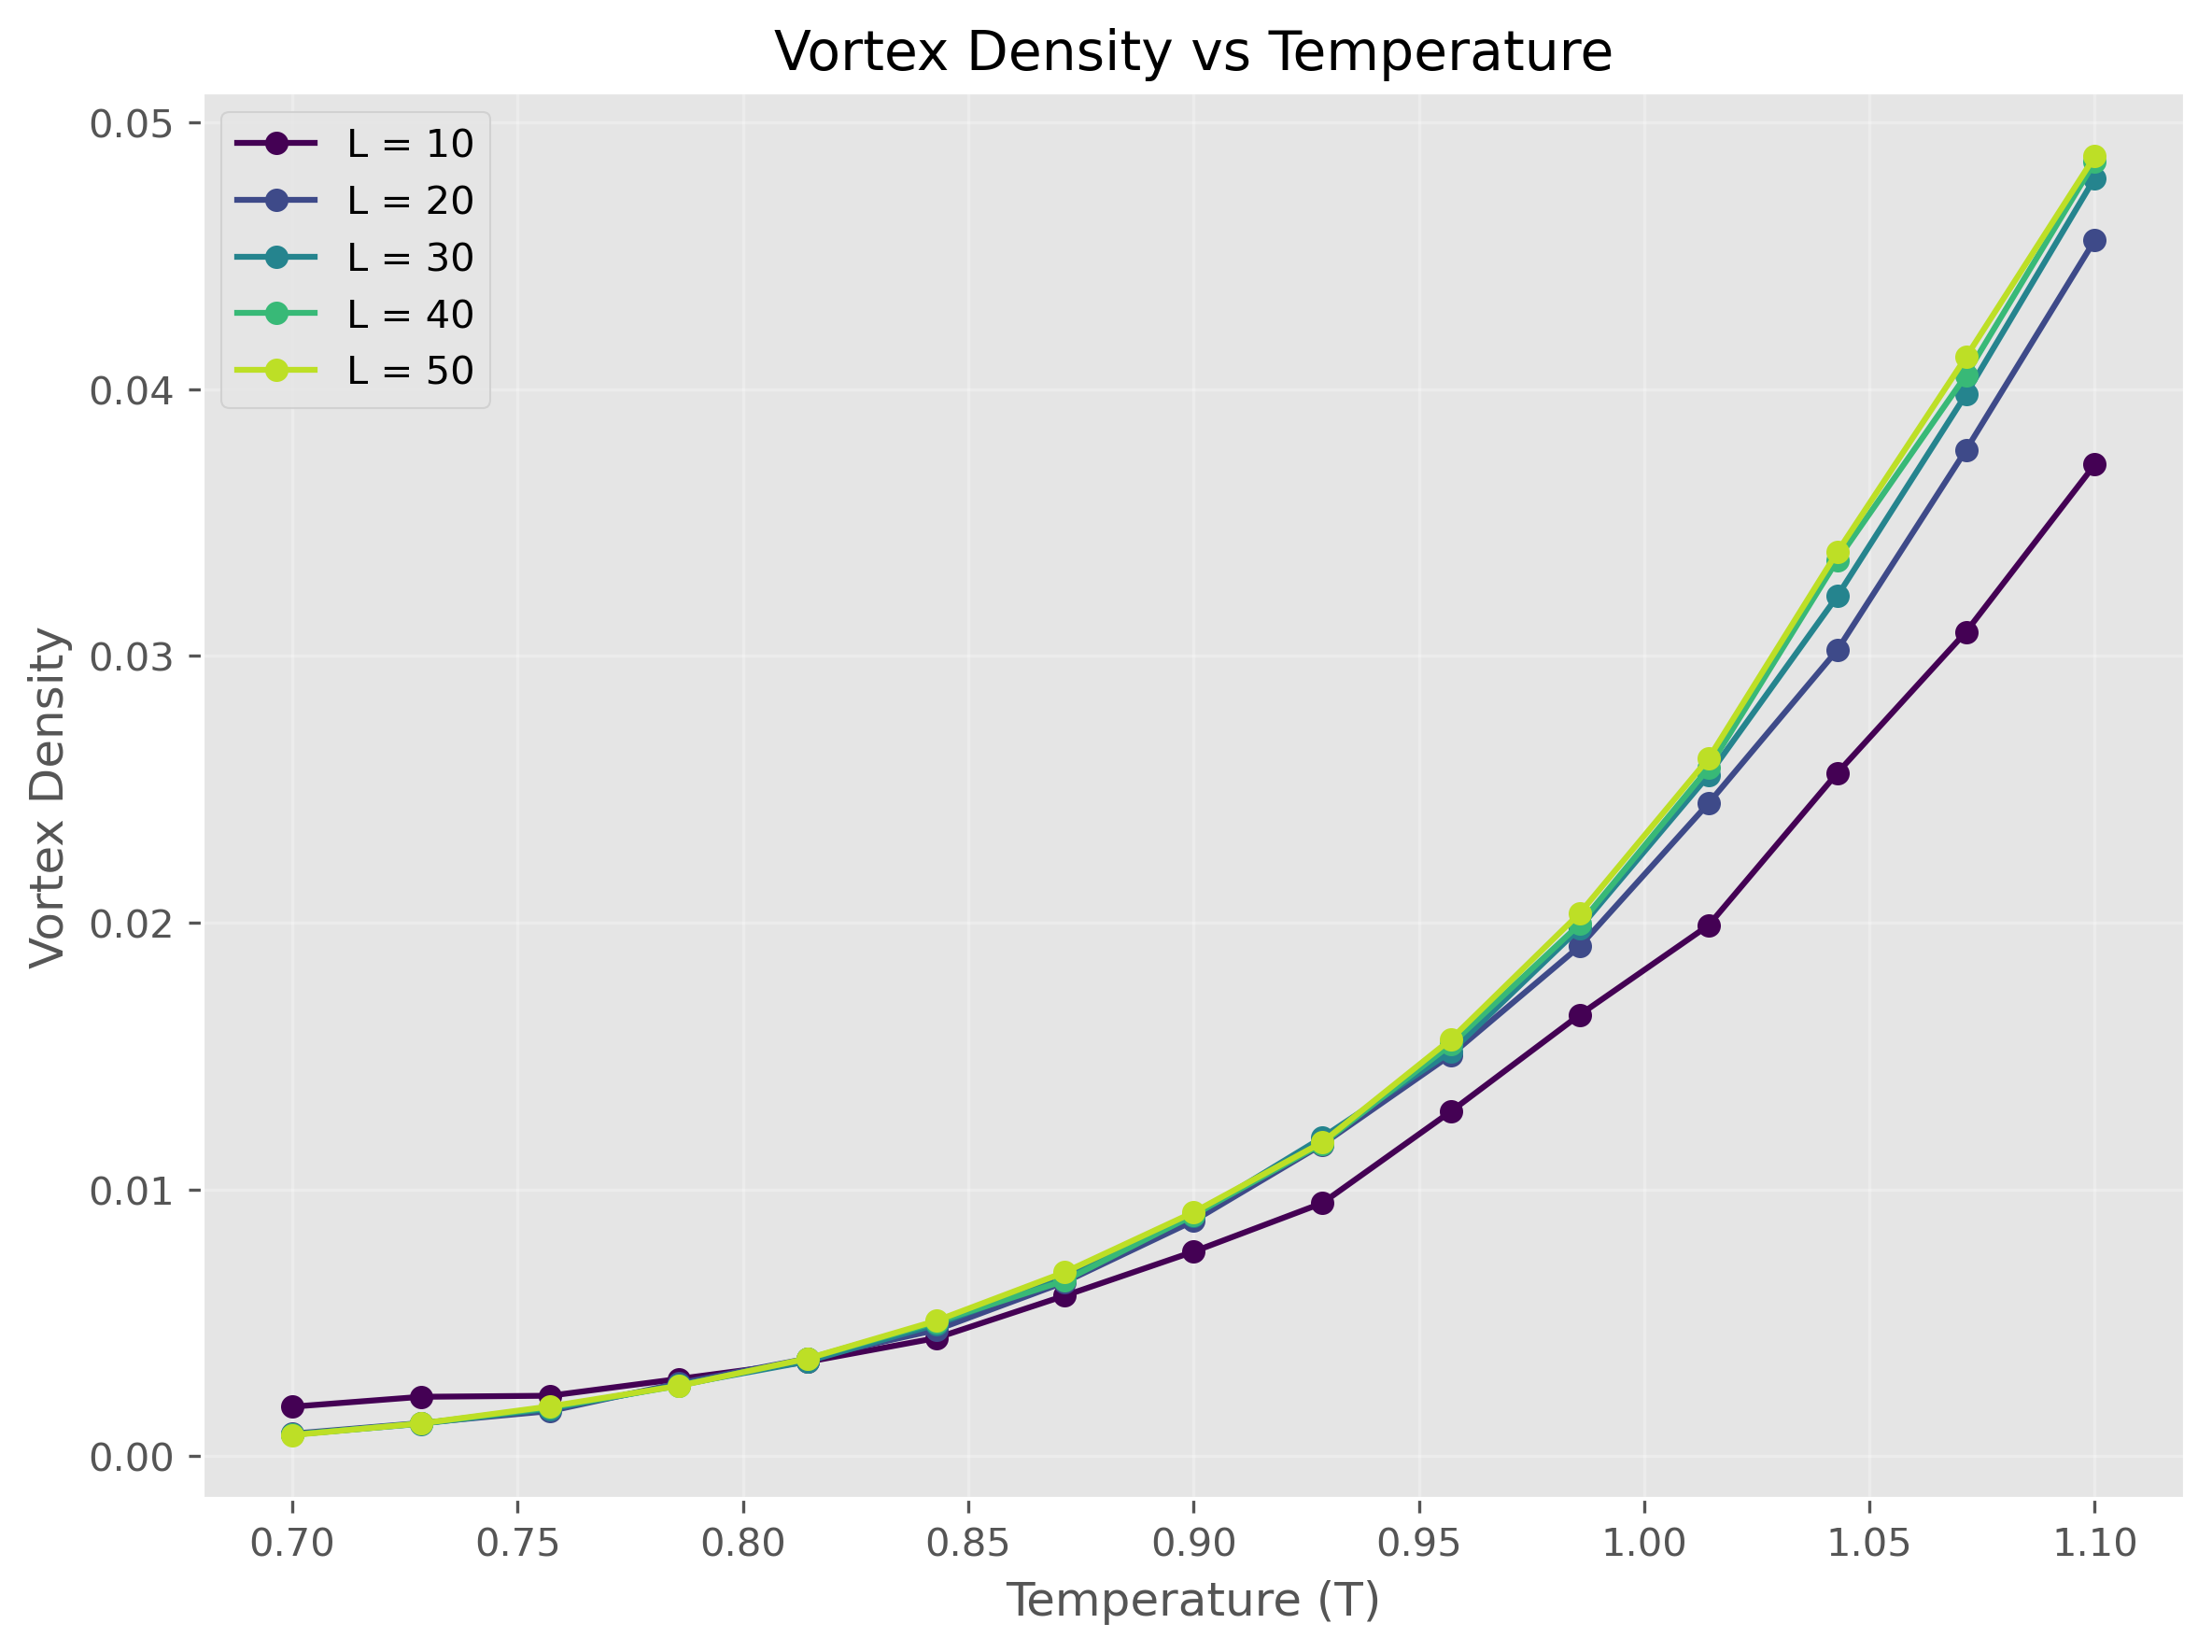
\includegraphics[width=0.95\linewidth]{images/observables/xy_model_vortices_wolff.png}
            % Remove the explicit vertical space
            % \vspace{0.5em}
            \centering % Center the caption text
            {\tiny Plot shows average vortex density vs $T$ for different $L$.}
        \end{column}
    \end{columns}
\end{frame}




\begin{frame}{Finite-Size Scaling of $T_{KT}(L)$}
    \begin{columns}[T] % Align columns at the top
        \begin{column}{0.55\textwidth}
            \textbf{Extracting the Transition Temperature}
            \begin{itemize}
                \item Estimate $T_{KT}(L)$ for each size $L$ from the intersection $\rho_s(T, L) = 2k_B T/\pi$.
                \item BKT theory predicts the scaling towards the thermodynamic limit ($L \to \infty$):
                \\[0.5em]
                $\qquad T_{KT}(L) = T_{KT}(\infty) + \frac{c}{(\ln(L/L_0))^2}$
                \\[0.5em]
                where $c$ and $L_0$ are non-universal constants.
                \pause
                \item Plotting $T_{KT}(L)$ vs $1/(\ln L)^2$ should yield a linear relationship for large $L$.
                \item The y-intercept gives the estimate for $T_{KT}(\infty)$.
                \pause
                \item Our linear fit yields:
                $\mathalert{T_{KT}(\infty) \approx 0.893(4) J / k_B}$
                \item Result is consistent with established literature values (e.g., Ref. \cite{drouin2022kosterlitz} and others cite $T_{KT} \approx 0.8928 J/k_B$).
            \end{itemize}
        \end{column}
        \begin{column}{0.45\textwidth}
             
\includegraphics[width=\linewidth]{images/scaling/xy_model_fss_wolff.png}
             \vspace{0.5em}
             {\tiny Plot shows $T_{KT}(L)$ extracted from stiffness data vs $1/(\ln L)^2$. The line is a linear fit.}
        \end{column}
    \end{columns}
\end{frame}



\begin{frame}{Finite-Size Scaling of $T_{KT}(L)$}
    \begin{columns}[T] % Align columns at the top
        \begin{column}{0.55\textwidth}
            \textbf{Extracting the Transition Temperature}
            \begin{itemize}
                \item Estimate $T_{KT}(L)$ for each size $L$ from the intersection $\eta(T, L) = 0.25$.
                \item BKT theory predicts the scaling towards the thermodynamic limit ($L \to \infty$):
                \\[0.5em]
                $\qquad T_{KT}(L) = T_{KT}(\infty) + \frac{c}{(\ln(L/L_0))^2}$
                \\[0.5em]
                where $c$ and $L_0$ are non-universal constants.
                \pause
                \item Plotting $T_{KT}(L)$ vs $1/(\ln L)^2$ should yield a linear relationship for large $L$.
                \item The y-intercept gives the estimate for $T_{KT}(\infty)$.
                \pause
                \item Our linear fit yields:
                $\mathalert{T_{KT}(\infty) \approx 0.893(4) J / k_B}$
                \item Result is consistent with established literature values (e.g., Ref. \cite{drouin2022kosterlitz} and others cite $T_{KT} \approx 0.8928 J/k_B$).
            \end{itemize}
        \end{column}
        \begin{column}{0.45\textwidth}
             
\includegraphics[width=\linewidth]{images/scaling/xy_model_fss_wolff_eta.png}
             \vspace{0.5em}
             {\tiny Plot shows $T_{KT}(L)$ extracted from decay exponent vs $1/(\ln L)^2$. The line is a linear fit.}
        \end{column}
    \end{columns}
\end{frame}



% --- Section 6: Conclusion ---
\section{Conclusion}

\begin{frame}{Summary and Significance}
    \begin{itemize}
        \item Successfully simulated the BKT transition in the 2D XY model:
        \begin{itemize}
            \item Implemented efficient Wolff algorithm with parallel tempering
            \item Measured key observables across multiple system sizes
            \item Applied finite-size scaling to extract critical temperature
        \end{itemize}
        \pause
        \item Key findings:
        \begin{itemize}
            \item Confirmed the characteristic signatures of the BKT transition
            \item Determined $T_{KT} \approx 0.893(4) J$ in good agreement with theory
            \item Observed universal jump in spin stiffness
            \item Demonstrated vortex unbinding mechanism
        \end{itemize}
        \pause
        \item Broader implications:
        \begin{itemize}
            \item BKT transition represents a unique universality class
            \item Demonstrates the power of topological defects in phase transitions
            \item Provides insight into universal mechanisms across diverse physical systems
            \item Highlights importance of advanced sampling techniques for critical phenomena
        \end{itemize}
    \end{itemize}
\end{frame}

\begin{frame}{Future Directions}
    \begin{itemize}
        \item Methodological improvements:
        \begin{itemize}
            \item Further optimization for larger system sizes
            \item GPU implementation for parallel computation
            \item Advanced analysis techniques for critical properties
        \end{itemize}
        \pause
        \item Extensions to related models:
        \begin{itemize}
            \item XY model with disorder or frustration
            \item Quantum XY models and quantum phase transitions
            \item Higher-dimensional models with topological transitions
        \end{itemize}
        \pause
        \item Applications:
        \begin{itemize}
            \item Superconducting thin films and arrays
            \item Quantum computing platforms based on 2D systems
            \item Cold atom experiments with vortex dynamics
            \item Theoretical connections to fundamental physics
        \end{itemize}
    \end{itemize}
\end{frame}

% --- Bibliography ---
\begin{frame}[allowframebreaks]{References}
    \printbibliography
\end{frame}

% --- Closing Slide ---
\begin{closingframe}

    \begin{center}
        \begin{minipage}{1\textwidth}

            \textbf{Lara Turgut}\hfill\textit{\email{lturgut@ethz.ch}}
            
            \vspace{0.25em}

            ETH Zurich, Department of Physics
            

            \vspace{0.5em}


            \textbf{Francesco Conoscenti}\hfill\textit{\email{fconoscenti@ethz.ch}}
            
            \vspace{0.25em}

            ETH Zurich, Department of Information Technology and Electrical Engineering
            

            \vspace{0.5em}


            \textbf{Ben Bullinger}\hfill\textit{\email{bben@ethz.ch}}

            \vspace{0.25em}

            ETH Zurich, Department of Computer Science

        \end{minipage}
    \end{center}

\end{closingframe}

\end{document}